%!TEX root = ../Technische Dynamik.tex

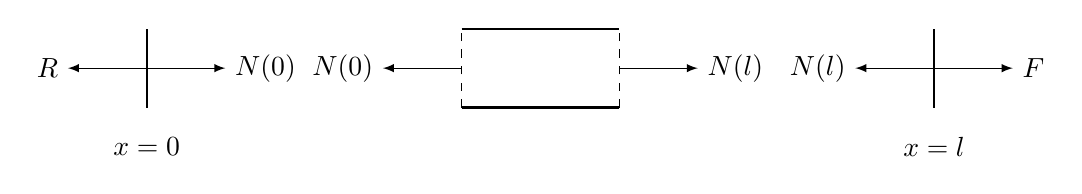
\begin{tikzpicture}[>=latex]
\begin{scope}
	\draw[thick] (0,0) -- (0,1);
	\draw[->] (0,0.5) -- (-1,0.5) node[left] {$R$};
	\draw[->] (0,0.5) -- (1,0.5) node[right] {$N(0)$};

	\node at (0,-0.5) {$x=0$};
\end{scope}

\begin{scope}[xshift=4cm]
	\draw[thick] (0,0) -- (2,0)
	                   (0,1) -- (2,1);
	\draw[dashed] (0,0) -- (0,1)
	                      (2,0) -- (2,1);

	\draw[->] (0,0.5) -- (-1,0.5) node[left] {$N(0)$};
	\draw[->] (2,0.5) -- (3,0.5) node[right] {$N(l)$};
\end{scope}

\begin{scope}[xshift=10cm]
	\draw[thick] (0,0) -- (0,1);
	\draw[->] (0,0.5) -- (-1,0.5) node[left] {$N(l)$};
	\draw[->] (0,0.5) -- (1,0.5) node[right] {$F$};

	\node at (0,-0.5) {$x=l$};
\end{scope}
\end{tikzpicture}